\chapter{Usecase}
\label{ch:usecase}
\cref{fig:foto_tureschliessanlage} zeigt eine Türschließanlage in welcher Form sie aktuell in Zügen der Intercity-Klasse von der Deutschen Bahn eingesetzt werden. Die Anlage wird durch einen pneumatischen Kolben angetrieben. Über eine Zahnstange treibt der Kolben ein Rad an, welches wiederum einen Bautenzug betätigt. Am einem Stahlseil, das über Seilrollen geführt wird, wird die Tür auf- bzw. zugezogen.

\begin{figure}[ht]
	\centering
	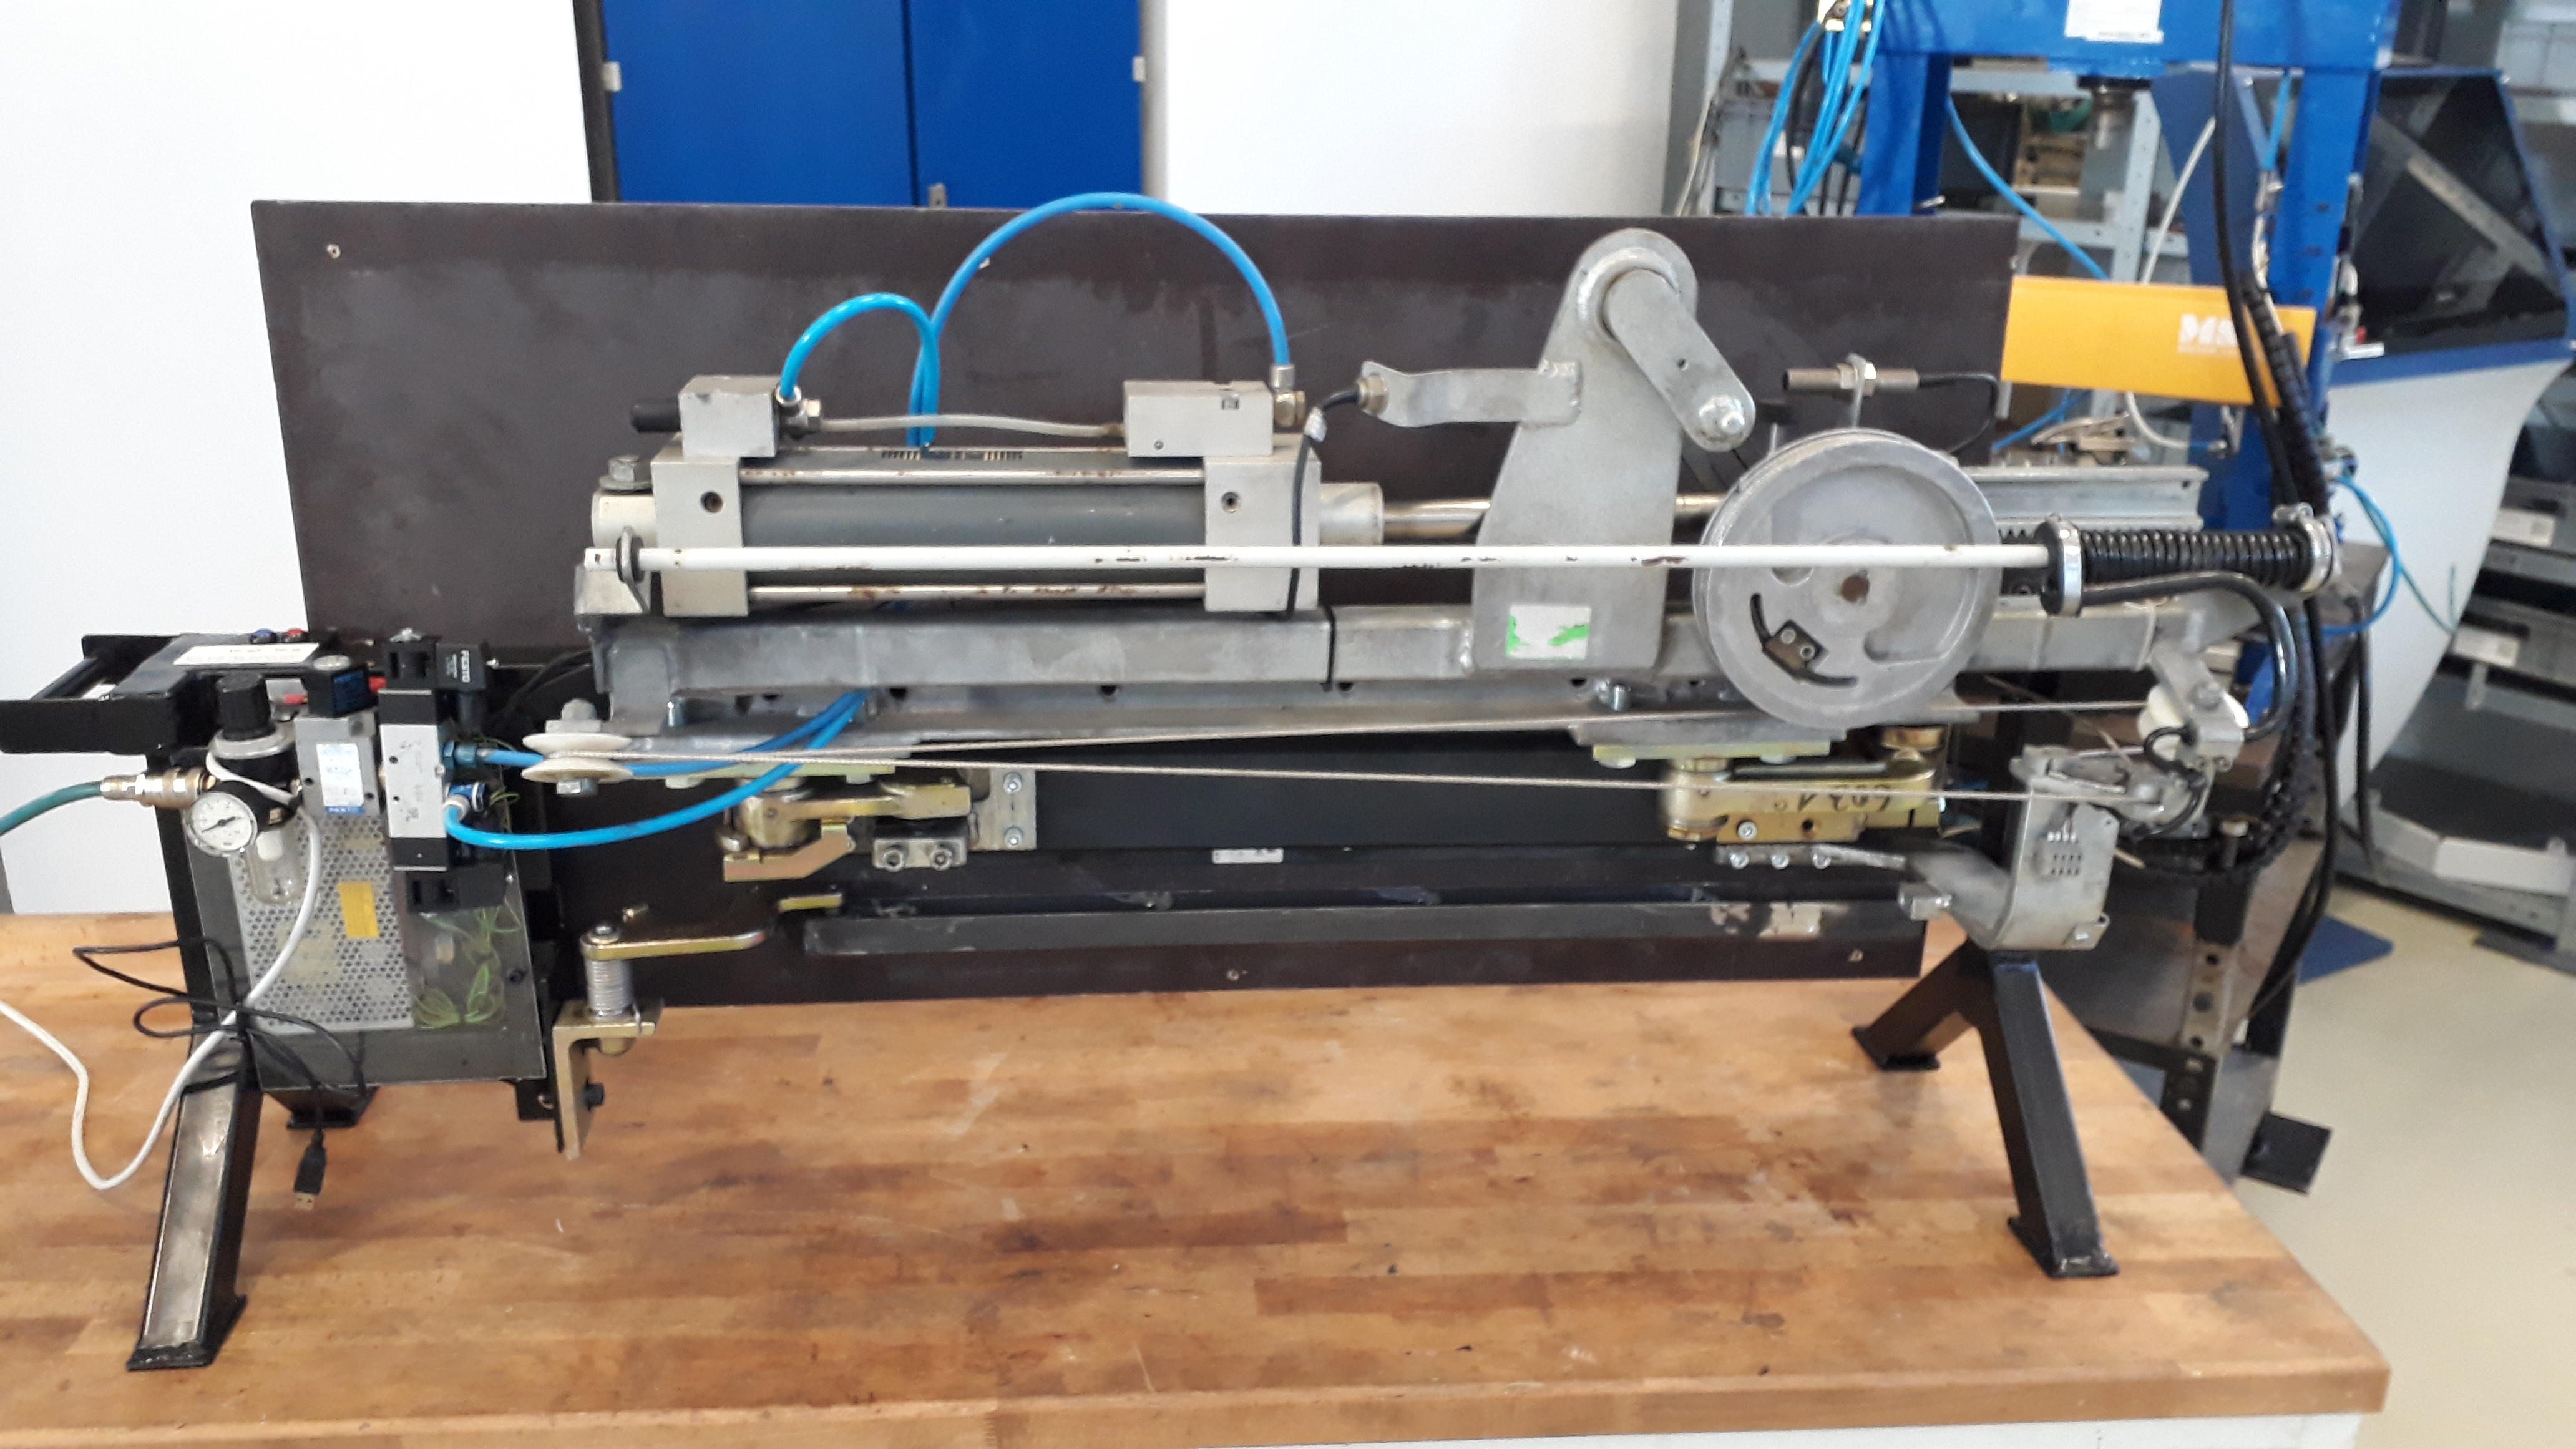
\includegraphics[width=\textwidth]{Foto_Türschließanlage.jpg}
	\caption{Ausgebaute Türschließanlage eines Zuges der Intercity-Klasse (Deutsche Bahn)}
	\label{fig:foto_tureschliessanlage}
\end{figure}

Wartungen der Anlage werden im Rahmen einer präventiven Instandhaltung durchgeführt. Zu diesem Zweck werden auch die Seilrollen regelmäßig ausgetauscht. Die Instandhaltungsmaßnahme wird entweder nach sechs Jahren oder nach \num{1.2} Millionen gefahrenen Kilometern durchgeführt~\cite{db.2021}.

Die Seilrollen aus Kunststoff sind ohne Wälzlager auf Bolzen montiert. Verschleiß und Materialermüdung sind in erster Linie an der Mantelfläche der Bohrung zu erwarten, an der die Rolle auf dem Bolzen aufliegt. Fortschreitende Rissbildung aufgrund von Materialermüdung bestimmt die Lebensdauer der Seilrollen. Mit steigendem Grad der Beschädigung steigt auch das Risiko eines Gewaltbruchs durch Überlast. In diesem Fall fällt die Türschließanlage aus und eine nicht planmäßige Instandsetzungsmaßnahme ist erforderlich.

Kann zu einem beliebigen Zeitpunkt der Zustand der Seilrollen bestimmt werden, so kann jederzeit der Bedarf einer Instandhaltungsmaßnahme eingeschätzt werden. Unerwartete Ausfällen können so vermieden werden (vgl. \cref{ch:instandhaltungsstrategien}). Kann der aktuelle Zustand darüberhinaus mit einem zu erwartendem Änderungsverlauf in Zusammenhang gebracht werden, kann sogar eine Vorhersage zum Ausfallzeitpunkt abgegeben werden. Die Vorteile einer prädiktiven Instandhaltung können so genutzt werden (vgl.~\cref{sec:praediktive_instandhaltung})

Die Instandhaltung der Seilrollen kann durch einem PdM-Ansatz gelöst werden. Voraussetzung dafür ist Erstens, dass Messwerte vorliegen, die Informationen über den Zustand der Seilrolle beinhalten. Zweitens sind diese Informationen in ein Entscheidungsmodel zu integrieren, das anhand von neuen Messwerten den Zustand der Rollen bestimmen kann. Drittens muss eine Infrastruktur geschaffen werden mit der in festgelegten Zeitabständen aktuelle Messwerte aufgenommen und verarbeitet werden können.
%===============================================================================
\section{Erfolgskriterien}
\label{sec:erfolgskriterien_usecase}
Um bestimmen zu können ob die Umstellung der Instandhaltung auf einen PdM-Ansatz sinnvoll ist, muss eine ausgiebige Nutzwertanalyse abgeschlossen und mit dem aktuell verwendetem Instandhaltungsansatz verglichen werden. 

Aufgrund der prinzipiell verschiedenen Natur von CM, PM und PdM, lassen sich nur wenige Vergleichende kriterien bestimmen. Beispielsweise kann die Anzahl vermeidbarer Ausfälle nicht verglichen werden, weil bei einem PM-Ansatz dazu keine Informationen zur Verfügung stehen. (Für die modelbewertung in \cref{ch:modelbewertung} entspricht eine beschädigte Seilrolle der Kategorie 1; ein nicht vermeidbarer Ausfall entspricht demnach einer \textit{falsch negativen} Vorhersage.) Auch werden bei PM per Definition keine unnötigen Inspektionen durchgeführt, wie es bei PdM für falsch positive Meldungen der Fall wäre. Um einen Vergleich der beiden Ansätze erheben zu können, sind also allgemeinere vergleichende Kriterien zu finden.

Im Rahmen dieser Arbeit wird ausschließlich auf Kriterien eingegangen, die den Nutzwert des vorgeschlagenen PdM-Ansatzes quantifizieren. Die Kriterien werden für die Bewertung der maschinellen Lernmodelle herangezogen, die in \cref{sec:modellierung} erstellt werden. Die folgenden Kriterien definieren den Nutzen der PdM-Anwendung.

\textbf{Komplexität}\\
Idealerweise soll das Modell nicht nur möglichst korrekte Vorhersagen über den Zustand der Seilrollen abgeben können, sondern auch Informationen extrahieren, die für Verbesserungen der Konstruktion verwendet werden können. Dafür ist ein Model nötig dessen Entscheidungverfahren nachvollziehbar ist. Ein zu komplexes Model kann nicht unter praktikablen Bedingungen ausgewertet werden. Aus diesem Grund ist ein einfach nachzuvollziehendes Model einem komplexeren vorzuziehen.

\textbf{Qualität der Vorhersagen}\\
Damit der Usecase einen Mehrwert gegenüber dem vorherigen Vorgehen bietet, müssen die Vorhersagen des Models ein Mindestmaß an Genauigkeit bieten können. Die Zahl falsch positiver, wie auch falsch negativer Vorhersagen (Fehlalarme bzw. unentdeckte Beschädigungen), sollten möglichst gering ausfallen. Ein Mindestmaß für beide Eigenschaften hängt von der Qualität des gegenüber stehenden PM-Usecases ab. Weil -- wie einleitend erwähnt -- dieses Kriterium keinen direkten Vergleich zwischen dem PM- und PdM-Ansatz zulässt, werden Annahmen für die Mindestmaße getroffen (s.~\cref{sec:bewertungskriterien}).

Bei der Qualität der Vorhersagen sind falsch positive Vorhersagen geringer zu wichten als falsch negative. Falsch positive Vorhersagen haben eine unnötige Inspektion oder Austausch der Komponente zufolge, wohingegen falsch negative Vorhersagen zu einem unerwarteten Ausfall führen. Im ersten Fall entstehen Kosten durch Verschwendung; im zweiten durch die notwendige Behebung einer Störung. Letzteres ist jedoch in der Regel mit höheren Kosten verbunden. Deswegen wird falsch negativen Vorhersagen ein höheres Gewicht zugeschrieben als falsch positiven Vorhersagen (s.~\cref{tab:paarvergleich}). Das Kriterium lässt sich in Form der Sensitivität und Relevanz direkt auf die Bewertung des verwendeten Vorhersagemodelle anwenden.
%===============================================================================
\section{Einordnung in den Kontext der Bahntechnik}
\label{sec:kontext_bahntechnik_von_usecase}
Der eröffnete Usecase beruht auf allgemeinen Prinzipien von PdM. Darüberhinaus gehend ist es sinnvoll den Usecase in den Kontext der praktischen Bahntechnik ein zu ordnen. Insbesondere eine Diskusion über den tatsächlichen Bedarf, als auch eine Darstellungen des angewandten Wartungsvorgehen ist für eine Bewertung des Usecases zuträglich.

Um den Usecase in den Kontext der Bahntechnik zu stellen, wurden zwei Interviews mit Sachverständigen der Deutschen Bahn und der Hochbahn Hamburg geführt. Die folgenden Abschnitte geben die wichtigsten Ergebnisse dieser Interviews wieder.
%===============================================================================
\subsection{Interview: Hochbahn Hamburg}
\label{subsec:interview_hochbahn}
\textit{Interview mit Jürgen Beck~\cite{hochbahn.2020} am {23.11.2020}}

Herr Beck benannte im Allgemeinen Lager als Komponenten, deren Wartungen von Kenntnissen über den aktuellen Zustand profitieren kann. Sie gehören zu den Komponenten, die dem größten Verschleiß unterworfen sind und daher häufig zu ersetzen sind. Die Seilrollen sind nicht in Verbindung mit einem Wälzlager montiert, sondern stützen sich direkt auf einem Bolzen ab. Verschleiß -- bedingt durch Relativbewegung zwischen Bolzen und Rolle -- tritt also an der Seilrolle selbst auf. Vor diesem Hintergrund ist die Wahl, die Seilrollen mit einem PdM-Ansatz instand zu halten, ebenso sinnvoll wie für Wälzlager.

Bezogen auf den Betrieb der Hochbahn in Hamburg wurde diskutiert welche Auswirkungen ein Ausfall der Türschließanlage hat und ob sich daraus ein Bedarf für den vorgeschlagenen Usecase ableiten lässt. Herr Beck betonte, dass eine Störung der Türanlage nur in Ausnahmefällen einen bedeutsamen Einfluss auf den Betriebsablauf hat. Für einen solchen Ausnahmefall müssten mehrere Türschließanlage an dem selben Waggon ausfallen und der Waggon dürfte nicht durch Zwischentüren mit den anhängenden Waggons verbunden sein. Nur in einem solchen Fall ist ein sicherer Betrieb des Waggons nicht mehr möglich, weil Fluchtmöglichkeiten unzulässig beschränkt sind. Es wird nicht erwartet, dass eine derartiger Ausnahmefall eine Umstellung der Instandhaltung auf einen PdM-Ansatz rechtfertigen kann. Dies ist der auch der Grund dafür warum die Hochbahn Hamburg aktuell nicht an der Umsetzung einer PdM-Anwendung arbeitet, wie sie zu Beginn dieses Kapitels vorgeschlagen wurde.
%===============================================================================
\subsection{Interview: Deutsche Bahn}
\label{subsec:interview_deutsche_bahn}
\textit{Interview mit Dr. Jörg Lehmann~\cite{db.2021} am {27.01.2021}}

Herr Lehmann beschrieb das Vorgehen der Deutschen Bahn bei der Instandhaltung von Regional- und Fernverkehrszügen wie folgt: Unterschieden wird zwischen der \textit{betriebsnahen} und der \textit{schweren} Instandhaltung. Die betriebsnahe Instandhaltung wird durch den Zugbetreiber durchgeführt und umfasst Instandhaltungsmaßnahmen, die die kurzfristige Verfügbarkeit des Zuges gewährleisten. Im Gegensatz zur schweren Instandhaltung, wird sie nach Bedarf durchgeführt. Neben Reinigungsarbeiten und Reparaturen an Interiör, umfasst sie auch Arbeiten an technischen Systemen des Zuges. Eine Türstörung kann laut Lehmann in der Regel im Rahmen einer betriebsnahen Instandhaltung behoben werden. Das bedeutet, dass Maßnahmen zur vorausschauenden Instandhaltung kurzfristig umgesetzt werden können, ohne dafür neue Strukturen schaffen zu müssen.

Die schwere Instandhaltung wird entweder nach sechs Jahren Betriebsdauer oder nach \num{1.2} Millionen gefahrenen Kilometern vorgenommen. Sofern die festgelegte Kilometeranzahl noch nicht erreicht ist, kann nach einer Einschätzung durch Sachverständige, das Intervall	auf \num{8} Jahre angehoben werden. Zu Beginn der schweren Instandhaltung wird eine Eingangsuntersuchung vorgenommen. Daran schließen sich Instandhaltungsmaßnahmen in Form von Plan-, Sicherheits- und Außerplanarbeiten an. Planarbeiten stehen bereits im Vorfeld der schweren Instandhaltung fest und werden grundsätzlich durchgeführt. Sicherheitsarbeiten werden umgesetzt, ohne dass es dafür einer extra Auftragsstellung bedarf. Außerplanarbeiten bedürfen hingegen einer nachträglichen Auftragsstellung. Die Auftragsstellungen erfolgen auf Basis der Ergebnisse der Eingangsuntersuchung. Gegeben dem Fall, dass durch die PdM-Anwendung Informationen über den Zustand der Seilrollen vorliegen, kann ihre Instandhaltung im Rahmen von Planarbeiten erledigt werden. Es wird also ein Zeitvorsprung gewonnen, der eine Planung ermöglicht.

Die Aussagen von Herrn Beck bezüglich des Bedarfs des Usecases teilt Herr Lehmann. Auch seiner Ansicht nach ist der Einfluss einer Türstörung auf den Betriebsablauf klein, weswegen wirtschaftlicher Mehrwert nicht zu erwarten sei.
%===============================================================================


